%%%%%%%%%%%%%%%%%%%%%%%%%%%%%%%%%%%%%%%%%
% Thin Sectioned Essay
% LaTeX Template
% Version 1.0 (3/8/13)
%
% This template has been downloaded from:
% http://www.LaTeXTemplates.com
%
% Original Author:
% Nicolas Diaz (nsdiaz@uc.cl) with extensive modifications by:
% Vel (vel@latextemplates.com)
%
% License:
% CC BY-NC-SA 3.0 (http://creativecommons.org/licenses/by-nc-sa/3.0/)
%
%%%%%%%%%%%%%%%%%%%%%%%%%%%%%%%%%%%%%%%%%

%----------------------------------------------------------------------------------------
%   PACKAGES AND OTHER DOCUMENT CONFIGURATIONS
%----------------------------------------------------------------------------------------

\documentclass[a4paper, 11pt]{article} % Font size (can be 10pt, 11pt or 12pt) and paper size (remove a4paper for US letter paper)

\usepackage{hyperref}
\usepackage[portuguese,english]{babel}
\usepackage[utf8]{inputenc}
\usepackage{float}

\usepackage{color} % for the notes
\usepackage{xcolor}
\usepackage[protrusion=true,expansion=true]{microtype} % Better typography
\usepackage{graphicx} % Required for including pictures
\usepackage{wrapfig} % Allows in-line images
\usepackage{tocloft}

\usepackage{mathpazo} % Use the Palatino font
\usepackage[T1]{fontenc} % Required for accented characters
\linespread{1.05} % Change line spacing here, Palatino benefits from a slight increase by default
\usepackage{etoolbox}
\newcommand{\nlp}{\textsc{nlp}}
\newcommand{\cn}{\textsc{cn}}
\newcommand{\aab}{\textsc{aa}}
\newcommand{\aai}{\textsc{Aa}}
\newcommand{\ontologiaa}{\textsc{o}ntologi\textsc{aa}}
\newcommand{\owl}{{\sc owl}}
\newcommand{\rdfi}{{\sc Rdf}}
\newcommand{\rdf}{{\sc rdf}}
%\newcommand{\paaineli}{P{\sc aa}inel}
\newcommand{\paaineli}{P{\bf \sc aa}inel}
\newcommand{\paainel}{p{\sc aa}inel}
\newcommand{\gsd}{\textsc{gsd}}
\newcommand{\ui}{\textsc{ui}}
%\newcommand{\lmb}{\url{lab\textsc{M}acambira.sf.net}}
\newcommand{\lm}{lab\textsc{M}acambira.sf.net}
%\newcommand{\lm}{\url{labMacambira.sf.net}}



\makeatletter
\renewcommand\@biblabel[1]{\textbf{#1.}} % Change the square brackets for each bibliography item from '[1]' to '1.'
\renewcommand{\@listI}{\itemsep=0pt} % Reduce the space between items in the itemize and enumerate environments and the bibliography

\hypersetup{
        colorlinks,
            linkcolor={red!50!black},
                citecolor={blue!50!black},
                    urlcolor={blue!80!black}
                }


\pretocmd{\chapter}{\addtocontents{toc}{\protect\addvspace{5\p@}}}{}{}
\pretocmd{\section}{\addtocontents{toc}{\protect\vspace{-4mm}}}{}{}
\renewcommand{\maketitle}{ % Customize the title - do not edit title and author name here, see the TITLE block below
\begin{flushright} % Right align
{\LARGE\@title} % Increase the font size of the title

\vspace{50pt} % Some vertical space between the title and author name

{\large\@author} % Author name
\\\@date % Date

\vspace{40pt} % Some vertical space between the author block and abstract
\end{flushright}
}

%----------------------------------------------------------------------------------------
%   TITLE
%----------------------------------------------------------------------------------------

\title{\textbf{The Algorithmic-Autoregulation essay}\\ % Title
%a natural collective focus\\on the collective being} % Subtitle
a collective and natural focus\\ on self-transparency} % Subtitle

\author{\textsc{Renato Fabbri} % Author
\\{\textit{IFSC/USP, Participa.br/SG-PR, labMacambira.sf.net}}} % Institution

\date{\today} % Date

%----------------------------------------------------------------------------------------

\begin{document}

\maketitle % Print the title section

%----------------------------------------------------------------------------------------
%   ABSTRACT AND KEYWORDS
%----------------------------------------------------------------------------------------

%\renewcommand{\abstractname}{Summary} % Uncomment to change the name of the abstract to something else


\begin{abstract}
    There are numerous pursues for a lightweight and systematic account of what is done by a group and containing individuals. The \aab\ (Algorithmic-Autoregulation) is a special case, in which a technical community embraced the challenge of registering their own dedication for sharing processes, self-transparency enhancements, and prove dedication. \aai\ is used since June/2011 by dozens of users, with the support of different software gadgets and for distinct tasks. Intermittence and activity concentration of users activity follows expected natural properties. Social participation and ontological understandings of \aab\ eases comparative analysis and furthers integration.
\end{abstract}

{
\selectlanguage{portuguese}
\begin{abstract}

\end{abstract}
}

\hspace*{3,6mm}\textit{Keywords:} distributed development, floss, social participation, OWL, statistics, anthropological physics % Keywords

%\vspace{30pt} % Some vertical space between the abstract and first section

%----------------------------------------------------------------------------------------
%   ESSAY BODY
%----------------------------------------------------------------------------------------
\newpage
\tableofcontents


\section{\aai\ start}\label{sec:start}
%\addcontentsline{toc}{section}{\aai\ start}
The Algorithmic Autorregulation (\aab) is a self-transparency mechanism for sharing processes, proving dedication, and enhance personal of collective self-transparency. Purposes for \aab\ usage are numerous: enable automated and fair compensation for dedications, ease co-working, introduce newcommers, and keeping public historical logs of activities, etc. Indeed, other systems have been designed for such a task (see Section~\ref{sec:rel}). A brief characterization of \aab\ is:
\begin{itemize}
    \item The collective origin, purpose and upkeep. This is a free-culture trait, present within many software, and leads to open software and data as described in Section ~\ref{sec:sdata}.
    \item Voluntary logging of messages about ongoing work.
    \item Aimed at coordinating distributed team work through individual merit.
    \item More a practice than a software: \aab\ presents variations on the software support and message composition. Often present are screencasts, peer validation and periodic messaging.
\end{itemize}

Transparency in this context should be understood as usual organization or State transparency is: a public account of activities~\cite{stso}; not directly as transparency in self-knowledge, as is the case in some philosophical and political contexts~\cite{stph}. One should reach~\cite{paaper} for a noteworthy overview of \aab\ as a Global Software Development (\gsd).

 \subsection{Related work}\label{sec:rel}
%\addcontentsline{toc}{subsection}{Related work}
 Authors know of no \emph{civil society transparency} platform. There is a number of transparency initiatives for governments~\cite{govTr}, for religious parties~\cite{espTr} and for private institutions~\cite{priTr}. Data analysis methods are derived from Natural Language Processing (\nlp) and Complex Networks (\cn) fields, constituting a hybrid framework of classical~\cite{cla1,cla2} and novel~\cite{nov1,nov2} approaches.

\subsection{Historical note}
7th June, 2013, Cleodon Silva~\cite{cleodon} died by heart failure. In his memory, the \lm\ group was born (Pedro Macambira was one of this pseudonyms). The \aab\ was conceived as the ``cardiac pulse'' of the group and is in constant usage since July, 2011. It gathers thousands of messages, tenths of users and hundreds of processes. \aai\ messages present contributions, such as  commits to official repositories of Evince, Firefox, OpenOffice, Puredata and other software~\cite{paaper}. Also, a number of other activities were registered: new software ellaboration and coding, writing of articles, wikis and etherpads; articulation of civil society, academic and State instances; studies and reviews. Even so, \aab\ is highly biased towards software development, as can be observed in Sections~\ref{sec:stats} and~\ref{sec:res}, and in the \gsd\ article about \aab~\cite{paaper}.

 \section{\aai\ Systems and data}\label{sec:sdata}
%\addcontentsline{toc}{section}{Systems and data}
 There are different software support for \aab\ (Section~\ref{sec:ss}). Also, distinct use methods are incident (Section~\ref{sec:sp}). This section exposes this diversity and their integration, as linked data, both within \aab\ variants and within participatory instances.

\subsection{Software support}\label{sec:ss}
There are mainly three software pieces written to support \aab\ activity. Two of them are a server and client suite each (see Sections~\ref{sec:aaFirst} and~\ref{sec:aa01}). The third is a fancy dashboard. Automated conversational agents (software [ro]bots) were used as alternative User Interfaces (\ui s), with a highlight for the Lalenia bot (see Section~\ref{sec:lalenia}), and an initiative to make \aab\ available in all chat networks (see Section~\ref{sec:ubi}).

All \aab\ software apparatus is contextualized in Table~\ref{tab:aas}.
\subsubsection{First \aab: server skin and shell client}\label{sec:aaFirst}
Although deprecated in favor of \aab\ 01, this first \aab\ software presents the most numerous set of functionalities. To understand them,
one needs to observe core design features:
\begin{itemize}
    \item
\end{itemize}

Client functionalities are:
\begin{itemize}
    \item
\end{itemize}

Server functionalities are:
\begin{itemize}
    \item
\end{itemize}

\begin{figure}[!h]
    \centering
    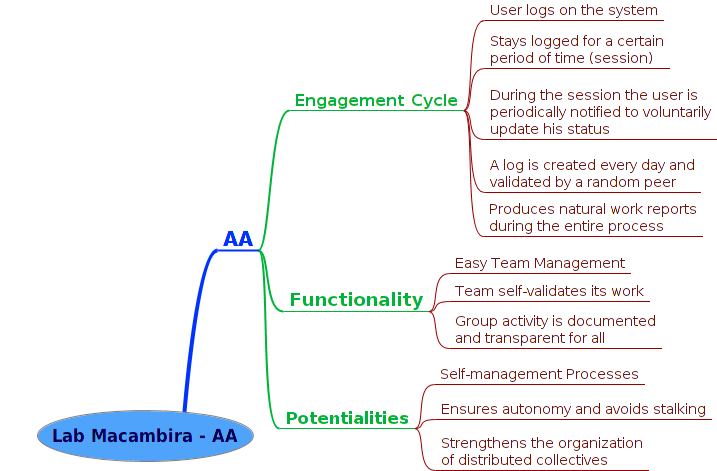
\includegraphics[width=\textwidth]{figs/aaFirstMethodology}
    \caption{A mind map of the AA methodology shared by users: i) Engagement cycle – the usage of AA; ii) Functionality – the design goals of the system; iii) Potentialities – envisioned benefits of AA by authors of the diagram. As seen in Section~\ref{sec:start}, core benefits emanate from the self-transparency aspect of~\aab, with worthy mentions to proving dedications and sharing processes.} 
    \label{fig:consult}
\end{figure}



Further information of this and other versions of \aab\ are contextualized in Table~\ref{tab:aas}.
\subsubsection{\paaineli}\label{sec:aaFirst}
\subsubsection{\aai\ 01}\label{sec:aa01}
\subsubsection{Lalenia interface}\label{sec:lalenia}
\subsubsection{Ubiquitous \aab}\label{sec:ubi}

%\addcontentsline{toc}{subsection}{Software support}
\begin{table}[!h]
  \centering
  \caption{All considered \aab\ versions and their databases.}\label{tab:aas}
  \begin{tabular}{|l|l|l|l|}\hline
{\bf version name} & {\bf main language} & {\bf user interface} & {\bf database} \\\hline\hline
& & & \\\hline
& & & \\\hline
& & & \\\hline
& & & \\\hline
& & & \\\hline
& & & \\\hline
& & & \\\hline
& & & \\\hline
& & & \\\hline
& & & \\\hline
& & & \\\hline
& & & \\\hline
  \end{tabular}
  \label{ospRestr}
\end{table}

\subsubsection{Messages in the \#labmacambira@Freenode IRC channel log}

\subsection{Systematic use proposals}\label{sec:sp}
%\addcontentsline{toc}{subsection}{Systematic use proposals}

\subsection{The \ontologiaa\ \owl\ ontology}
%\addcontentsline{toc}{subsection}{The \ontologiaa\ \owl\ ontology}

\subsection{\rdfi\ data}
%\addcontentsline{toc}{subsection}{\rdfi\ data}

\subsection{Linkage to other participatory data}
%\addcontentsline{toc}{subsection}{Linkage to other participatory data}


\section{Statistics}\label{sec:stats}
%\addcontentsline{toc}{section}{Data statistics}

\section{Results}\label{sec:res}

\section{Conclusions}
\subsection{Further work}
%\addcontentsline{toc}{subsection}{\ontologiaa: the \aab\ ontology}
%\begin{wrapfigure}{l}{0.4\textwidth} % Inline image example
%\begin{center}
%\includegraphics[width=0.38\textwidth]{telao1.png}
%\end{center}
%\caption{\small Telão para streaming de estruturas sociais, usado no \#arenaNETmundial, \#ocupaGOV e outras ocasiões. Tela com rede de retweets e relacionamento via hashtag e vocabulário. Atualizada a cada 10 segundos com os relacionamentos implicados pelos dos tweets mais recentes.}\label{fig:telao}
%\end{wrapfigure}

%\begin{figure}[H]
%  \centering
%    \includegraphics[width=.7\textwidth]{telao2.png}
%  \caption{\small Telão para streaming de estruturas sociais, usado no \#arenaNETmundial, \#ocupaGOV e outras ocasiões. Tela com relacionamentos de hashtags e vocabulário. Atualizada a cada 10 segundos com conteúdo dos tweets mais recentes.}\label{fig:telao2}
%\end{figure}










%----------------------------------------------------------------------------------------
%   BIBLIOGRAPHY
%----------------------------------------------------------------------------------------

%\bibliographystyle{unsrt}
%\bibliographystyle{plain}
\bibliographystyle{ieeetr}
\bibliography{ensaio}

%----------------------------------------------------------------------------------------

\end{document}
